% This file was converted to LaTeX by Writer2LaTeX ver. 1.0.2
% see http://writer2latex.sourceforge.net for more info
\documentclass[a4paper]{article}
\usepackage[utf8]{inputenc}
\usepackage[T3,T1]{fontenc}
\usepackage[slovene,english,french]{babel}
\usepackage[noenc]{tipa}
\usepackage{tipx}
\usepackage[geometry,weather,misc,clock]{ifsym}
\usepackage{pifont}
\usepackage{eurosym}
\usepackage{amsmath}
\usepackage{wasysym}
\usepackage{amssymb,amsfonts,textcomp}
\usepackage{color}
\usepackage{array}
\usepackage{supertabular}
\usepackage{hhline}
\usepackage{hyperref}
\hypersetup{pdftex, colorlinks=true, linkcolor=black, citecolor=black, filecolor=black, urlcolor=black, pdftitle=OpenWIM, pdfauthor=Ivan, pdfsubject=, pdfkeywords=}
\usepackage[pdftex]{graphicx}
\usepackage[alf,utf8,recuo=8pt]{abntex2cite}


% Text styles
\newcommand\textstyletablecaptionCar[1]{\foreignlanguage{english}{\textbf{#1}}}
% Outline numbering
\setcounter{secnumdepth}{2}
\renewcommand\thesection{\arabic{section}}
\renewcommand\thesubsection{\arabic{section}.\arabic{subsection}}
\makeatletter
\newcommand\arraybslash{\let\\\@arraycr}
\makeatother
% List styles
\newcommand\liststyleWWNumvi{%
\renewcommand\theenumi{\arabic{enumi}}
\renewcommand\theenumii{\arabic{enumii}}
\renewcommand\theenumiii{\arabic{enumiii}}
\renewcommand\labelitemi{[F0B7?]}
\renewcommand\labelenumi{\theenumi.}
\renewcommand\labelenumii{\theenumii.}
\renewcommand\labelenumiii{\theenumiii.}
}
% Page layout (geometry)
\setlength\voffset{-1in}
\setlength\hoffset{-1in}
\setlength\topmargin{2.501cm}
\setlength\oddsidemargin{2.501cm}
\setlength\textheight{24.698002cm}
\setlength\textwidth{15.999001cm}
\setlength\footskip{0.0cm}
\setlength\headheight{0cm}
\setlength\headsep{0cm}
% Footnote rule
\setlength{\skip\footins}{0.119cm}
\renewcommand\footnoterule{\vspace*{-0.018cm}\setlength\leftskip{0pt}\setlength\rightskip{0pt plus 1fil}\noindent\textcolor{black}{\rule{0.25\columnwidth}{0.018cm}}\vspace*{0.101cm}}
% Pages styles
\makeatletter
\newcommand\ps@Standard{
  \renewcommand\@oddhead{}
  \renewcommand\@evenhead{}
  \renewcommand\@oddfoot{}
  \renewcommand\@evenfoot{}
  \renewcommand\thepage{\arabic{page}}
}
\makeatother
\pagestyle{Standard}
\setlength\tabcolsep{1mm}
\renewcommand\arraystretch{1.3}
% footnotes configuration
\makeatletter
\renewcommand\thefootnote{\arabic{footnote}}
\makeatother

%\bibliographystyle{plain}
\bibliographystyle{abntex2-alf}

\def\citeay#1{\citeauthor{#1} (\citeyear{#1})} % Super!!!!!

\title{Universidade Federal de Santa Catarina}
\author{Ivan Ogassavara}
\date{2016-02-14}
\begin{document}
\clearpage\setcounter{page}{1}\pagestyle{Standard}
{\centering\selectlanguage{english}\bfseries
OpenWIM - Open Science and Weigh-in-Motion Research
\par}


\bigskip

\begin{flushleft}
\tablehead{}
\begin{supertabular}{m{3.8749998cm}m{3.8760002cm}m{3.8760002cm}m{3.8749998cm}}
\selectlanguage{english} Tecnólogo pesquisador graduado pela Faculdade Eniac, especializado em Sistemas de Informação pelo Centro de Pós-Graduação Eniac. Experiência em algoritmos para estimação de peso de veículos em movimento. &


\includegraphics[width=2.619cm,height=3.307cm]{openwim-img/openwim-img1.png}
 &

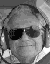
\includegraphics[width=2.619cm,height=3.307cm]{openwim-img/openwim-img2.png}
 &
\selectlanguage{english} Engenheiro pesquisador graduado pela PUC-RJ, especializou-se em planejamento de transportes urbanos pela \textit{Massachusetts Institute of Technology - MIT}. Também foi um dos pioneiros da área de pesagem de veículos pesados no Brasil, atuando desde 1974 nesse tema.\\
\multicolumn{2}{m{7.951cm}}{\centering
{\selectlanguage{english}\bfseries Ivan Ogassavara}\par

\centering {\selectlanguage{english} Universidade Federal de Santa Catarina}\par

\centering \selectlanguage{english} Brazil} &
\multicolumn{2}{m{7.951cm}}{\centering
{\selectlanguage{english}\bfseries Helio Goltsman}\par

\centering {\selectlanguage{english} Universidade Federal de Santa Catarina}\par

\centering \selectlanguage{english} Brazil}\\
\end{supertabular}
\end{flushleft}

\bigskip


\bigskip

{\selectlanguage{english}\bfseries
Abstract}

{\selectlanguage{english}

Overweight heavy vehicles represent a big problem related to accidents and pavement damage. The weight enforcement is very important to inhibit the overweight of these vehicles. One method that is being investigated in many parts of the world is weigh-in-motion (WIM), which has the advantage of reduced physical space and operating costs. Since the sensors can be installed on the road itself, it can weigh passing vehicles, without them having to slow down, hence, not delaying the road user’s journey.

Although there are many papers publicly available about weigh-in-motion in the engineering transportation area, there has not been much research based on free access sources and data or including explanations that allow the reproduction of results. In this context, the Open Science concept can help improve the WIM research through collaborative efforts and reproducible methods, using algorithms and data with free public access.

The OpenWIM project was born upon this background as an Open Science initiative, to provide a WIM research repository with initial structure based on the main information available in the literature. This can then be converted into a framework for researchers to develop and test new methods and technologies.

The structure of this project was designed over some pillars:
\begin{itemize}
\item Standards;
\item Open Data;
\item Reproducibility;
\item Algorithms;
\item Papers.
\end{itemize}

The Standards pillar is based on a recompilation of standards found in the international literatures used in WIM projects. This can be a guideline to new researchers to structure their projects and can facilitate the shared used of data and algorithms. This standards can be about the file names, layout data structure, file format used in system integration, standard units, column name standard (in data files), algorithms style code, etc.

The Open Data pillar is based on a open repository where Weigh-in-Motion data is published. This data can be:

\begin{itemize}
\item Raw data from weigh sensors;
\item Raw data from inductive loop;
\item Known information about the vehicle run (gross vehicle weight, speed, distance between axles, weight in each axle, vehicle category, temperature, etc.);
\item Vehicle category patterns;
\item Calibration data;
\item License plate images;
\item Vehicle images;
\end{itemize}

The raw data from sensors and the weight information is very important to validate weigh and calibration methods. Raw data from inductive loop can help in methods like vehicle classification. The license plate images can help to test or improve methods that recognizes the plate position and license value. The vehicle images can be used, for example, by vehicle classification method using image processing and artificial neural network.

The Reproducibility pillar is based on Notebook Sciences to describe and explain about some method, data or concept related to Weigh-in-Motion. This slope will use the Jupyter Notebook technology as default tool. With this tool, the researcher can write texts, texts with latex format, and algorithms; open data files; plot charts; display tables; show images; etc. Jupyter Notebooks can be used with some main programming languages like Python, Julia, Octave, Matlab, Bash, Scheme, etc.

The Algorithms pillar is based on a repository for researchers public his algorithms used in their research. This algorithms with a test dataset can help other researchers in their research that allows more alternatives in their experiences. Other important key about this pillar is the informal peer-review because when other researchers can test some algorithms they can find some problem or exception.

The "main product" of academic and scientific environments are the Papers. The Papers pillar is based on a collaborative environment that allows researchers of all parts of the world to work together in some research. When a researcher has some interesting in a specific research that can join to this group to sum efforts in that project. This can be used to handle economic limitations.

}


\bigskip

{\selectlanguage{english}
The papers will be first published in the conference proceedings, later
on the ISWIM website, and the best ones may be submitted to a Journal
with the authors' agreement.}


\bigskip

{\selectlanguage{english}
\textstyletablecaptionCar{Keywords:} \ Heavy
Vehicles, Weigh-in-Motion, WIM, Open Science, Open Data, Reproducibility.}


\bigskip

{\selectlanguage{english}\bfseries
\foreignlanguage{portuguese}{Resumo}}

{\selectlanguage{english}
\foreignlanguage{portuguese}{
Resumo...
}}


\bigskip

{\selectlanguage{english}
\textstyletablecaptionCar{\foreignlanguage{portuguese}{Palavras-Chaves:}}\foreignlanguage{portuguese}{
Veículos Pesados, Pesagem em Movimento, WIM, Ciência Aberta, Dados Abertos, Reprodutibilidade}}

\section{Introduction}
{\selectlanguage{english}
In \citeonline{kistler2004installation}, ....

\iffalse

\section{Figures, Tables, and Equations}
{\selectlanguage{english}
All figures, tables, and equations should be numbered consecutively by
type and referenced within the text, e.g., Figure 1, Table 1, Equation
(1). \ They should be placed in the paper as near as possible after the
point at which they are first mentioned. The words “figure,” “table,”
and “equation” may not be abbreviated.}

\subsection{Figures}
{\selectlanguage{english}
Figures include illustrations, photographs, charts, and graphs. All
figures should be given captions. \ Captions should be centered beneath
the figure, and all words (except articles and prepositions) should be
capitalized (see example below). Separate captions from body text with
one line space. }


\bigskip

{\selectlanguage{english}
Figure caption should be in 11-point Times New Roman. The name
“\textbf{Figure N -}” should be in bold.}


\bigskip

{\centering 
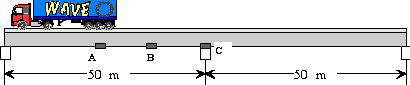
\includegraphics[width=12.277cm,height=2.566cm]{openwim-img/openwim-img3.pdf}
\par}

{\centering\selectlanguage{slovene}\bfseries
Figure 1 – This is a sample figure caption
\par}


\bigskip

{\selectlanguage{english}
All writing within figures should, where possible, be in 10.5-point
Times New Roman. Please note that color images will be printed in black
and white in the paper proceedings and must remain understandable. }

\subsection{Tables}
{\selectlanguage{english}
Table captions should be above the table, flush left, and in 11-point
Times New Roman. \ Separate table captions from body text and the table
with one line space above and below the captions as below. \ }


\bigskip

{\selectlanguage{english}\bfseries
Table 1 - Summary statistics for pre-weighed trucks (COV = Coefficient
of Variance)}


\bigskip

\begin{flushleft}
\tablehead{}
\begin{supertabular}{|m{2.799cm}|m{2.052cm}|m{2.0509999cm}|m{2.0509999cm}|m{2.0509999cm}|m{2.0509999cm}|m{1.7969999cm}|}
\hline
~
 &
\multicolumn{2}{m{4.3030005cm}|}{\centering \selectlanguage{english}
Type 1} &
\multicolumn{2}{m{4.302cm}|}{\centering \selectlanguage{english} Type 4}
&
\multicolumn{2}{m{4.0480003cm}|}{\centering \selectlanguage{english}
Type 5}\\\hline
~
 &
\centering \selectlanguage{english} Gross &
\centering \selectlanguage{english} Axle &
\centering \selectlanguage{english} Gross &
\centering \selectlanguage{english} Axle &
\centering \selectlanguage{english} Gross &
\centering\arraybslash \selectlanguage{english} Axle\\\hline
\selectlanguage{english} Mean IF &
\centering \selectlanguage{english} 1.00 &
\centering \selectlanguage{english} 0.98 &
\centering \selectlanguage{english} 1.03 &
\centering \selectlanguage{english} 1.03 &
\centering \selectlanguage{english} 1.02 &
\centering\arraybslash \selectlanguage{english} 1.02\\\hline
\selectlanguage{english} COV (\%) &
\centering \selectlanguage{english} 7.21 &
\centering \selectlanguage{english} 9.86 &
\centering \selectlanguage{english} 6.21 &
\centering \selectlanguage{english} 8.44 &
\centering \selectlanguage{english} 5.18 &
\centering\arraybslash \selectlanguage{english} 7.85\\\hline
\selectlanguage{english} Within 15\% &
\centering \selectlanguage{english} {}-{}-{}-{}-{}- &
\centering \selectlanguage{english} 93 &
\centering \selectlanguage{english} {}-{}-{}-{}-{}- &
\centering \selectlanguage{english} 94 &
\centering \selectlanguage{english} {}-{}-{}-{}-{}- &
\centering\arraybslash \selectlanguage{english} 85\\\hline
\end{supertabular}
\end{flushleft}

\bigskip

{\selectlanguage{english}
Tables should use 1-point lines for the top and bottom, and a half-point
line beneath the table’s header. \ Thickness of all table lines must be
0.5 point. All writing within tables should, where possible, be in
11-point Times New Roman. Cells’ content should be centered as much as
possible if relevant.}

\subsection{Equations and Units}
{\selectlanguage{english}
All equations should be indented 1.2 cm from the left margin and
numbered in brackets in the extreme right hand side of the page as
follows:}


\bigskip

{\selectlanguage{english}
\ \ \textit{C}\ \ =\ \ 
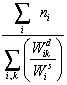
\includegraphics[width=2.011cm,height=2.54cm]{openwim-img/openwim-img4.pdf}
\ \ \ \ \ \ \ \ \ \ \ \ \ \ \ \ (2)}

\fi

\begin{small}
\renewcommand{\bibname}{References}
\addcontentsline{toc}{section}{\bibname}
\bibliography{openwim}
\end{small}

\end{document}
